\usetikzlibrary{shapes, calc, shapes, arrows, positioning}

\tikzstyle{neuron}=[draw,circle,minimum size=20pt,inner sep=0pt, fill=white]
\tikzstyle{stateTransition}=[thick]
\tikzstyle{learned}=[text=red]

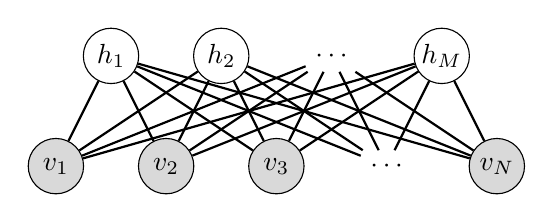
\begin{tikzpicture}[scale=1.4]
    \node (v1)[neuron, fill=gray!30] at (0, 0) {$v_1$};
    \node (v2)[neuron, fill=gray!30] at (1, 0) {$v_2$};
    \node (v3)[neuron, fill=gray!30] at (2, 0) {$v_3$};
    \node (vdots) at (3, 0) {$\cdots$};
    \node (v4)[neuron, fill=gray!30] at (4, 0) {$v_N$};
    % \node[right=0.1cm of v4] (v) {$\textbf{v} \in \{0, 1\}^N$};
    % \node[learned,below=0.1cm of v1] (bv1) {$b_{v_1}$};
    % \node[learned,below=0.1cm of v2] (bv2) {$b_{v_2}$};
    % \node[learned,below=0.1cm of v3] (bv3) {$b_{v_3}$};
    % \node[learned,below=0.1cm of v4] (bv4) {$b_{v_4}$};

    \node (h1)[neuron] at (0.5, 1) {$h_1$};
    \node (h2)[neuron] at (1.5, 1) {$h_2$};
    \node (hdots) at (2.5, 1) {$\cdots$};
    \node (h3)[neuron] at (3.5, 1) {$h_M$};
    % \node[right=0.1cm of h3] (h) {$\textbf{h} \in \{0, 1\}^M$};
    % \node[learned,above=0.1cm of h1] (bh1) {$b_{h_1}$};
    % \node[learned,above=0.1cm of h2] (bh2) {$b_{h_2}$};
    % \node[learned,above=0.1cm of h3] (bh3) {$b_{h_3}$};

    % \node[learned] (W) at (3.5, 0.5) {$W \in \mathbb{R}^{3 \times 4}$};

    % \draw[learned,stateTransition] (v1) -- (h1) node [midway,above=-0.06cm,sloped] {$w_{1,1}$};
    \draw[stateTransition] (v1) -- (h1) node [midway,above=-0.06cm,sloped] {};
    \draw[stateTransition] (v1) -- (h2) node [midway,above=-0.06cm,sloped] {};
    \draw[stateTransition] (v1) -- (hdots) node [midway,above=-0.06cm,sloped] {};
    \draw[stateTransition] (v1) -- (h3) node [midway,above=-0.06cm,sloped] {};

    \draw[stateTransition] (v2) -- (h1) node [midway,above=-0.06cm,sloped] {};
    \draw[stateTransition] (v2) -- (h2) node [midway,above=-0.06cm,sloped] {};
    \draw[stateTransition] (v2) -- (hdots) node [midway,above=-0.06cm,sloped] {};
    \draw[stateTransition] (v2) -- (h3) node [midway,above=-0.06cm,sloped] {};

    \draw[stateTransition] (v3) -- (h1) node [midway,above=-0.06cm,sloped] {};
    \draw[stateTransition] (v3) -- (h2) node [midway,above=-0.06cm,sloped] {};
    \draw[stateTransition] (v3) -- (hdots) node [midway,above=-0.06cm,sloped] {};
    \draw[stateTransition] (v3) -- (h3) node [midway,above=-0.06cm,sloped] {};

    \draw[stateTransition] (vdots) -- (h1) node [midway,above=-0.06cm,sloped] {};
    \draw[stateTransition] (vdots) -- (h2) node [midway,above=-0.06cm,sloped] {};
    \draw[stateTransition] (vdots) -- (hdots) node [midway,above=-0.06cm,sloped] {};
    \draw[stateTransition] (vdots) -- (h3) node [midway,above=-0.06cm,sloped] {};

    \draw[stateTransition] (v4) -- (h1) node [midway,above=-0.06cm,sloped] {};
    \draw[stateTransition] (v4) -- (h2) node [midway,above=-0.06cm,sloped] {};
    \draw[stateTransition] (v4) -- (hdots) node [midway,above=-0.06cm,sloped] {};
    % \draw[learned,stateTransition] (v4) -- (h3) node [midway,above=-0.06cm,sloped] {$w_{4,3}$};
    \draw[stateTransition] (v4) -- (h3) node [midway,above=-0.06cm,sloped] {};

\end{tikzpicture}
